\chapter{Design}
\section{Data Flow Diagram}
A data flow diagram is a graphical representation of the "flow" of data through an information system, modelling its process aspects. A DFD is often used as a preliminary step to create an overview of the system without going into great detail, which can later be elaborated. DFD's can be used for the visualization of data processing.
\par
Data flow diagrams are also known as bubble charts. DFD is a designing tool used in the top-down approach to system design. This context-level DFD is next "exploded", to produce a level-1 DFD that shows some of the detail of the system being modeled. The Level-1 DFD shows how the system is divided into subsystems, each of which deals with one or more of the data flows to from an external agent, and which together provide all of the functionality of the system as a whole. It also identifies internal data stores that must be present in order for the system to do its job, and shows the flow of data between the various parts of the system.

\begin{center}
\begin{figure}[H]
\centering
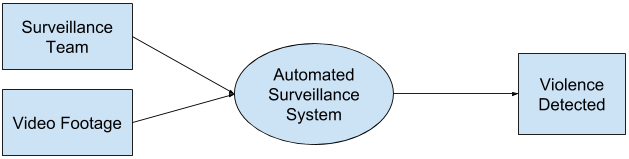
\includegraphics[width = \linewidth]{dfd0.png}
\caption{Data Flow Diagram Level 0}
\end{figure}
\end{center}

\begin{center}
\begin{figure}[H]
\centering
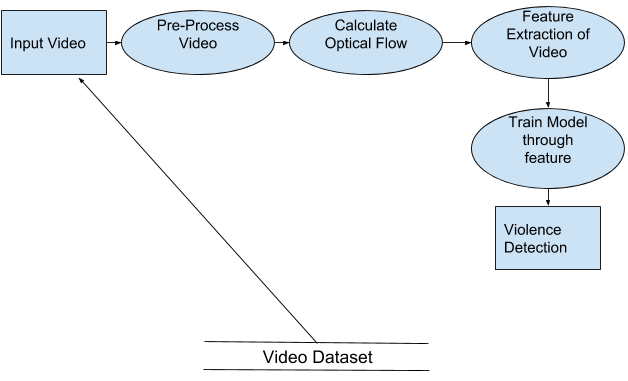
\includegraphics[width = \linewidth]{dfd1.png}
\caption{Data Flow Diagram Level 1}
\end{figure}
\end{center}

\section{UML Diagrams}
UML stands for Unified Modeling Language. UML is a standardized general-purpose modeling language in the field of object-oriented software engineering. The standard is managed, and was created by, the Object Management Group. 
\par
The UML is a very important part of developing objects oriented software and the software development process. The UML uses mostly graphical notations to express the design of software projects.\\
\subsection{Building blocks of UML}
The vocabulary of the UML encompasses three kinds of building blocks.
\begin{enumerate}
	\item Things.
	\item Relationships.
	\item Diagrams.
\end{enumerate}
\subsection{Things in UML}
Things are the abstractions that are first-class citizen in a model.\\
There are four kinds of things in the UML.
\begin{enumerate}
	\item Structure things.
	\item Behavioural things.
	\item Grouping things.
	\item Annotational things.
\end{enumerate}
These things are the basic object-oriented building blocks of the UML. You use them to write well-formed models.
\subsection{Relationships in the UML}
Things can be connected to logically be physically with the help of relationship in object oriented modelling.These are four kinds of relationships in the UML.

\begin{enumerate}
	\item Dependency.
	\item Association.
	\item Generalization.
	\item Realization.
\end{enumerate}
\subsection{Diagrams in UML}
A diagram is a graphical representation of a set of elements. These are nine kinds of diagrams in the UML.
\begin{enumerate}
	\item Class diagram.                 
\item  Object diagram                
\item  Use Case diagram.               
\item  Sequence diagram.             
\item  Collaboration diagram.
\item  Activity diagram.
\item  Component diagram.
\item  State chart diagram.
\item  Deployment diagram.

\end{enumerate}
\subsection{Component Diagram}
Automated Surveillance and Alert Generation System has the following components:
\begin{enumerate}
	\item OpenCV
	\item Bob
	\item Video Preprocess
	\item Optical Flow
	\item Violent Feature Extract
\end{enumerate}
\begin{center}
\begin{figure}[H]
\centering
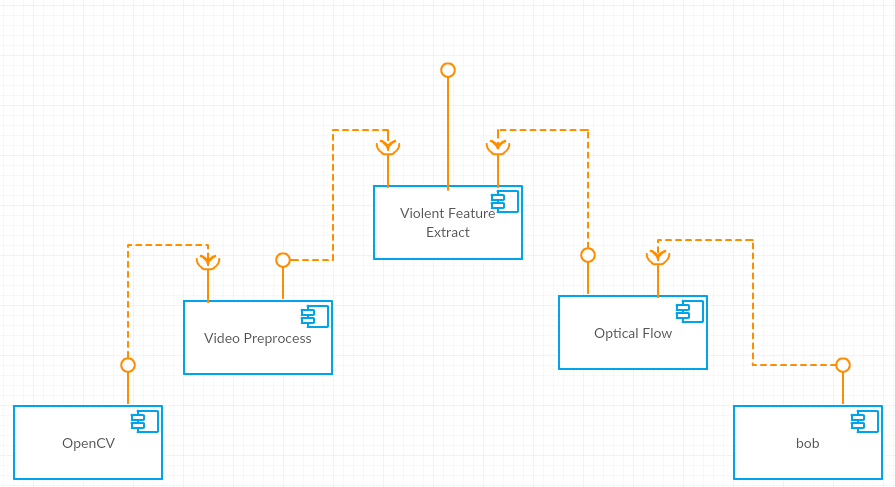
\includegraphics[width = \linewidth]{component.png}
\caption{Component Diagram}
\end{figure}
\end{center}
\subsubsection{OpenCV}
OpenCV (short for Open Computer Vision) is a package originally written in C language but later it was ported to Python. OpenCV possesses a rich set of interfaces and functions  that help us to read and manipulate video files. OpenCV can read video from input cameras and also from attached cameras to the system. Given a source of CCTV footage , through OpenCV we are able to manipulate frame size, the colour and the frame intervals. Video Preprocessing has to be done so that the further components can work at real-time which is on and average 1/25 th of a second for a frame.
\subsubsection{Bob}
Bob is a signal processing and machine learning platform available for python. Bob is provided as a precompiled source for Linux or Mac OS through Anaconda package manager. Bob helps us to port the signal processing procedures which are initially written in C language. Signal processing methods are usually written in C language as it can make native function calls and kernel function calls. So as to port these procedures into Python bob platform is used. C Liu’s Optical Flow algorithm [5] is being ported here through bob.
\subsubsection{Video Preprocess}
This is a self written Python library. It Preprocesses the video according to our needs. This library makes the necessary calls from the OpenCV so as to do the pixel level manipulations. Frame by Frame access is done by through this package. Frame interval is set as 3, default frame rate is taken as 25, each frame is resized to 100 pixel width and corresponding height. Frame is further converted into grayscale.
\subsubsection{Optical Flow}
This is also a self written package. It contains the procedures to calculate Optical flow which further call procedures from bob platform. Optical flow will return 3 things in a tuple, velocity along x , y axis and the wrap. This calculation is done by considering some pre calculated parameters.
\subsubsection{Video Feature Extract}
At a considered moment, three frames are under consideration. Previous frame , current frame and the next frame. First thing we do is we preprocess these frames and then calculated optical flows between successive frames. Now we have two optical flow vectors, now we calculate the absolute change between these two vectors. Average of this change vector is calculated and it is stored as threshold. Now the change vector is quantised with binary 1 and 0 by comparing it with threshold vector. This binary vector is summed for the whole video and normalized by dividing it with the number of iterations done till now. Binary vector generated till now is divided into (4 * 4) parts. For each of these parts , a histogram is built which has the bin size of 0.05 ranging from 0 to 1. Frequency of each bin is calculated and normalized by dividing with sum of all frequencies. Now all of the normalized histograms are appended one after another and the resulting vector is known as \textit{Violent Feature Vector}.